\section{Dataset Collection}

We use the Stack Exchange Data
Explorer\footnote{\texttt{https://data.stackexchange.com/stackoverflow/query/new}}
and construct a custom SQL query on the Stack Overflow data. The query could be
found under \texttt{source\_code/query.sql}.

The query satisfies the three requirements:

\begin{itemize}
    \item \texttt{\ldots select top 500} means that we are collecting at least
    500 threads.
    \item \texttt{\ldots Tags like \textquotesingle{}\%python\%\textquotesingle{}}
    means that we are collecting threads tagged \texttt{python}, discussing the
    Python programming language.
    \item \texttt{\ldots where AnswerCount >= 1} means we are collecting
    threads with at least 1 question and 1 answer.
\end{itemize}

The dataset contains 500 questions and 1254 answers, an average of 2.508 answers
per question. The distribution of answers is shown in Figure~\ref{ans-dist}.

\begin{figure}[h]
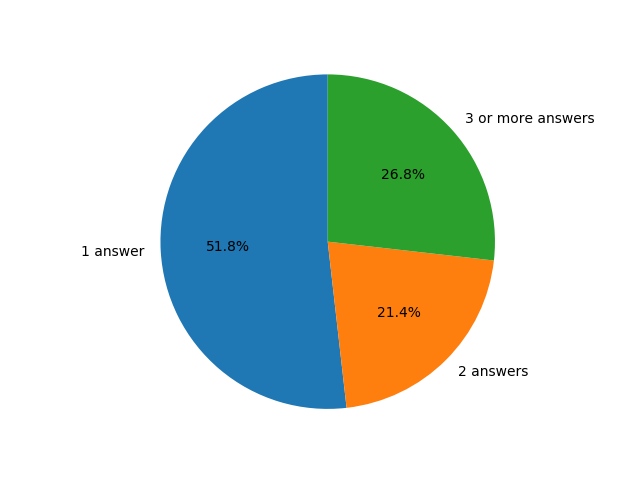
\includegraphics[width=0.9\linewidth]{no_ans_per_qn}
\caption{Distribution of answers}\label{ans-dist}
\end{figure}

\section{Dataset Analysis and Annotation}

\section{Tokenizer}

\section{Further Analysis and Annotation}

\section{Application}